% geDIG v4 (English Draft)
% XeLaTeX build (arXiv note: \pdfoutput is only for pdfTeX)
\documentclass[12pt]{article}
\usepackage[utf8]{inputenc}
\usepackage[T1]{fontenc}
\usepackage{lmodern}
\usepackage{amsmath,amssymb,graphicx,booktabs}
\usepackage{amsthm}
\usepackage{algorithm}
\usepackage{algpseudocode}
\usepackage{tikz}
\usetikzlibrary{arrows.meta,positioning,calc,shapes.geometric}
\usepackage[hidelinks]{hyperref}
\usepackage[nameinlink]{cleveref}
\usepackage{microtype}
\usepackage{siunitx}
\usepackage{enumitem}
\usepackage[table]{xcolor}
\usepackage{float}
\usepackage[a4paper,margin=1in]{geometry}
\graphicspath{{figures/}{docs/paper/figures/}}

% Build switch: ignore missing figures when compiling
\makeatletter
\newif\iffigs
\figstrue
\iffigs\else
  \renewcommand{\includegraphics}[2][]{\rule{0pt}{0pt}}
\fi
\makeatother

% Theorems
\newtheorem{proposition}{Proposition}[section]
\newtheorem{theorem}{Theorem}[section]
\newtheorem{lemma}{Lemma}[section]
\newtheorem{corollary}{Corollary}[section]

% Macros
\newcommand{\F}{\mathcal{F}}
\newcommand{\gednorm}{\Delta\mathrm{EPC}_{\mathrm{norm}}}
\newcommand{\ignorm}{\Delta\mathrm{IG}_{\mathrm{norm}}}
\newcommand{\experimNote}[1]{\textcolor{red}{\textbf{[TBD: #1]}}}

\title{geDIG: A One-Gauge Framework for Controlling Dynamic Knowledge Graphs}
\author{Kazuyoshi Miyauchi\\ \small\texttt{miyauchikazuyoshi@gmail.com}}
\date{Draft (v4, English)}

\begin{document}
\maketitle

\begin{abstract}
We propose geDIG, a single-gauge ($\F$) control framework for dynamic knowledge graphs that unifies structure cost (normalized edit path cost, $\Delta$EPC) and information gain (entropy decrease and path shortening, $\Delta$IG). The two-stage gating (AG: attention, DG: decision) drives acceptance/rejection/exploration/backtrack/eviction in an event-driven manner, with a clean separation between 0-hop novelty/error detection (FEP-side) and multi-hop compression/shortcuts (MDL-side) for practical anytime operation. We adopt PSZ (Perfect Scaling Zone; Acc/FMR/latency SLO) as an \emph{operational target}; in our lightweight, reproducible runs we do not fully enter the PSZ band, but we observe consistent improvements in the PSZ shortfall and provide explicit AG/DG logs that make decisions auditable. We present results-first summaries for four experiments: (I) a partial-observation maze PoC, (II) static RAG baselines, (III) dynamic GRAG with PSZ analysis, and (IV) insight-vector alignment. Finally, we formulate an operational FEP--MDL bridge and give a thermodynamic reading (free energy) of $\F$.
\end{abstract}

\section{Introduction}
We study when and how to accept, connect, and reuse new knowledge episodes in a dynamic knowledge graph (KG). Our core hypothesis: a single numerical gauge $\F$ can reliably drive both learning (curation) and inference (retrieval/use).

\paragraph{One-Gauge and Two-Stage Gates}
We define once and use the short form thereafter:
\begin{equation}
  \ignorm := \Delta H_{\mathrm{norm}} + \gamma\,\Delta\mathrm{SP}_{\mathrm{rel}},\quad
  \F = \gednorm - \lambda\,\ignorm,
\end{equation}
where $\lambda$ sets the information temperature and $\gamma$ balances entropy vs path-efficiency. AG (attention) triggers on high 0-hop novelty/error; DG (decision) commits only when multi-hop gain is confirmed (shortcuts/compression).

\paragraph{Contributions (short)}
\begin{itemize}[leftmargin=1.2em]
  \item Results-first, unified control: $\F$ and two-stage gates for online acceptance/search/eviction.
  \item Static and dynamic RAG: clean split; dynamic metrics (PSZ, FMR) isolated in the Dynamic chapter.
  \item Operational FEP–MDL bridge and a free-energy reading of $\F$ (engineering, not identity).
\end{itemize}

\section{Design: One Gauge and Two-Stage Gating}
\subsection{0-hop vs Multi-hop: FEP and MDL}
0-hop evaluates draft wiring at the query hub (novelty/error; FEP-side), while multi-hop evaluates shortcuts/compression on induced subgraphs (MDL-side). Let $g_0 = \Delta\mathrm{EPC}_{\mathrm{norm}} - \lambda\,\Delta H_{\mathrm{norm}}$ and $g_{\min}=\min_h\{\Delta\mathrm{EPC}_{\mathrm{norm}}-\lambda(\Delta H_{\mathrm{norm}}+\gamma\,\Delta\mathrm{SP}_{\mathrm{rel}}^{(h)})\}$. AG fires if $g_0>\theta_{\mathrm{AG}}$; DG fires if $\min\{g_0,g_{\min}\}\le\theta_{\mathrm{DG}}$.

\subsection{Thermodynamic Reading (Metaphor)}
We can read $\F$ as an operational free energy:
\begin{equation}
  U := \Delta\mathrm{EPC}_{\mathrm{norm}} - \lambda\,\gamma\,\Delta\mathrm{SP}_{\mathrm{rel}},\quad S := \Delta H_{\mathrm{norm}},\quad F := U - \lambda S,\label{eq:free_energy_en}
\end{equation}
so $\F$ is isomorphic to $F$ by term rearrangement. The coefficient $\lambda$ plays the role of information temperature. We keep later references in the short form $\F=\gednorm-\lambda\,\ignorm$ to avoid redundancy.

\subsection{Evaluation Common Conditions}\label{sec:common_setup_en}
\footnote{For quick reproduction, see Make targets (e.g., \texttt{make exp23-paper}, \texttt{make maze-suite}) and the smoke script \texttt{scripts/codex\_smoke.sh}.}
We compare static and dynamic RAG under \emph{shared} conditions. Chapters only state their differences; definitions and resources live here.
\begin{itemize}[leftmargin=1.6em]
  \item \textbf{Knowledge source / Retriever / LM}: same corpus, retriever, and generation settings (prompt, temperature, max tokens).
  \item \textbf{Measurements}: answer quality (EM/F1), faithfulness (citation/Path Faithfulness), latency (P50; measured). In dynamic runs we also report contamination (FMR; over accepted events), PSZ (Acc/FMR/P50 SLO) with shortfall $s_{PSZ}$, and zero-hop rate (ZSR; no AG firing).
  \item \textbf{Equal resources}: embedder/ANN/Top-$k$/LLM/temperature/tokens/HW/parallelism/measurement held constant; a compact table is provided in the supplement.
  \item \textbf{Splits and calibration}: train/val/test with gates calibrated on val and fixed on test.
\end{itemize}

\begin{figure}[H]
  \centering
  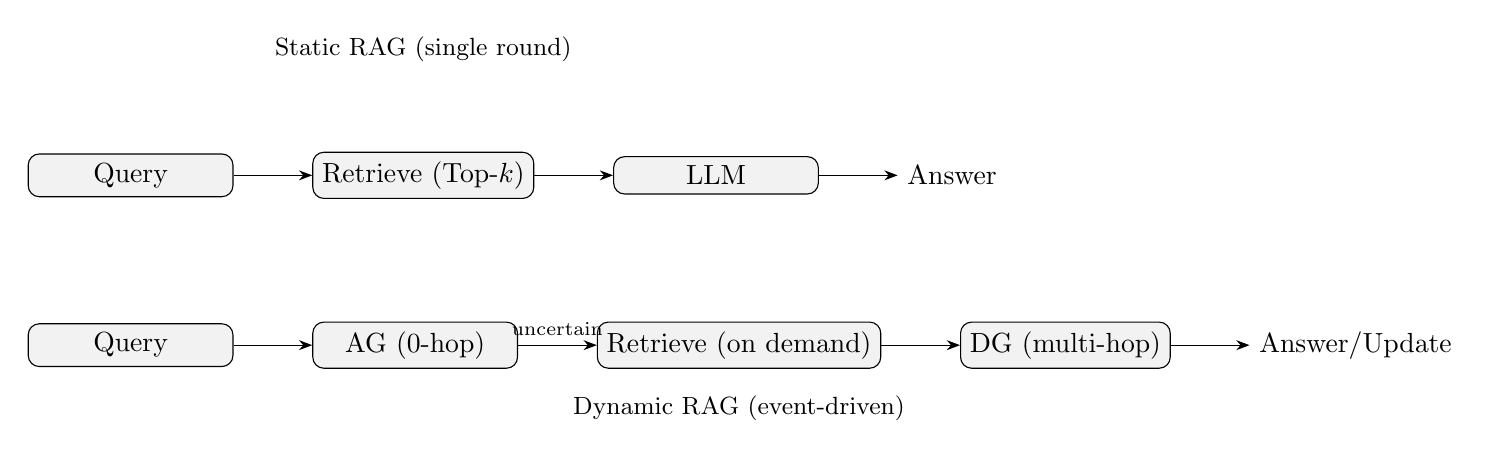
\begin{tikzpicture}[node distance=10mm,>=Stealth,rounded corners]
    % Static pipeline
    \node[draw,fill=gray!10,minimum width=26mm] (q1) {Query};
    \node[draw,fill=gray!10,minimum width=26mm,right=of q1] (r1) {Retrieve (Top-$k$)};
    \node[draw,fill=gray!10,minimum width=26mm,right=of r1] (l1) {LLM};
    \node[right=of l1] (a1) {Answer};
    \draw[->] (q1) -- (r1);
    \draw[->] (r1) -- (l1);
    \draw[->] (l1) -- (a1);
    \node[above of=r1,yshift=6mm,font=\small] {Static RAG (single round)};
    % Dynamic pipeline
    \node[draw,fill=gray!10,minimum width=26mm,below=16mm of q1] (q2) {Query};
    \node[draw,fill=gray!10,minimum width=26mm,right=of q2] (ag) {AG (0-hop)};
    \node[draw,fill=gray!10,minimum width=26mm,right=of ag] (r2) {Retrieve (on demand)};
    \node[draw,fill=gray!10,minimum width=26mm,right=of r2] (dg) {DG (multi-hop)};
    \node[right=of dg] (a2) {Answer/Update};
    \draw[->] (q2) -- (ag);
    \draw[->] (ag) -- node[above,font=\scriptsize]{uncertain} (r2);
    \draw[->] (r2) -- (dg);
    \draw[->] (dg) -- (a2);
    \node[above of=r2,yshift=-18mm,font=\small] {Dynamic RAG (event-driven)};
  \end{tikzpicture}
  \caption{Static (single-round) vs dynamic (event-driven) RAG pipeline. Dynamic triggers retrieval only when uncertain and updates on DG confirmation.}
  \label{fig:static_dynamic_pipeline_en}
\end{figure}

\section{Experiment I: Maze PoC (results-first)}
\paragraph{Summary} geDIG achieves large reductions in exploration ratio and revisit rate, with short backtracks and near-immediate dead-end detection. Example (25×25): \experimNote{exploration 0.38, revisit 1.28, backtrack 4.3, detection 0.8, success 100\%}.

\paragraph{Metrics} Primary: exploration ratio (unique/total), revisit (steps/unique), avg backtrack (AG→DG), dead-end detection delay, success rate. Secondary: Regret, SPL.

\paragraph{Success Criteria} Necessary: success\,$\ge$\,95\%, AG 5–10\%, DG 2–5\%, DG/AG 30–50\%, threshold stability (train/val within 2\%). Sufficient: exploration\,$\le$\,0.40, revisit\,$\le$\,1.5, backtrack\,$\le$\,5, detection\,$\le$\,1 with significance vs Greedy Novelty (Welch+Bonferroni, $p{<}0.01$, $d{>}0.5$). Diagnostic: Regret median\,$\le$\,+5, SPL mean\,$\ge$\,0.85.

\paragraph{Baselines (same conditions)} Greedy Novelty, $\varepsilon$-greedy, UCB1-like, Partially-Observed A*, and ablations (EPC-only / IG-only / no AG/DG / 0-hop only). Dijkstra/A* used as upper-bound diagnostics.

\section{Experiment II: RAG Baselines (static only)}
\paragraph{Summary} Under equal-resources, geDIG-soft (G1) improves EM/F1 by \experimNote{+2–5pt} over GT-RAG (B2), increases citation/path faithfulness by \experimNote{+5–10pt}, with comparable P50/P95 latency.

\paragraph{Baselines} B0: Flat RAG (SBERT, HNSW, Top-k), B1: GraphRAG (GNN), B2: Graph Transformer, G1: B2 + geDIG-soft (sigmoid$\,(\tau\F)$ for weighting/pruning/ordering). Static-only here; dynamic is in Experiment III. See Section~\ref{sec:common_setup_en} for common evaluation conditions and equal-resource assumptions.

\paragraph{Dataset and Protocol} 50 domains (mix of single-domain, cross-domain 2/3-hop, analogical). Sources: HotpotQA/2Wiki + curated. Equal-resources table (embedder/ANN/Top-k/LLM/temp/tokens/HW/parallelism/measurement) fixed across methods. No-peeking: train (burn-in for thresholds) / val / test split; thresholds fixed on val.

\section{Experiment III: Dynamic GRAG × geDIG}
\paragraph{Summary} With geDIG-soft applied consistently to retrieval/integration/summarization (G2), Temporal Consistency improves by \experimNote{+5–10pt}, update lag remains comparable or lower, KG contamination (FMR) decreases, and PSZ points emerge.

\paragraph{Dynamic Metrics} Temporal Consistency, update lag (ingest→available), KG contamination rate (FMR, rolling), 0-hop rejection, AG/DG rates (cf. Section~\ref{sec:common_setup_en}). PSZ: Acc\,$\ge$\,95\%, FMR\,$\le$\,2\%, extra P50\,$\le$\,200ms.

\paragraph{Time-Series and Operating Curves} Plot $\Delta$EPC/$\Delta H$/\,$\Delta$SP/$\F$ with acceptance time-series (pending→confirmed, C-value), and Operating Curves (Acc–FMR–Latency) with PSZ band.

\section{Experiment IV: Insight-Vector Alignment}
\paragraph{Summary} Readout vectors from DG-confirmed subgraphs align with LLM answer embeddings: \experimNote{$\Delta s{=}{+}0.2x$, $p{<}0.0x$, $N{=}200$}. Baselines: random, Top-k, threshold, AG-selected.

\section{FEP–MDL Bridge (operational proposition)}
\paragraph{Definition} We call an operational correspondence a relation that (i) is proportional (not identical), (ii) has a bounded residual $O(1/N)$ under assumptions, and (iii) yields testable predictions. Under mild assumptions (normalization, bounded horizon, decomposable edits, stable entropy estimation), $\F\propto\Delta\mathrm{MDL}+O(1/N)$. The coefficient $\lambda\approx c_D/c_M$ anchors scales.

\paragraph{Implications} A single control signal justifies simultaneous control of structure edits and inference. EPC on the structure side and IG on the information side avoid double counting. Ablations corroborate the roles of $\Delta H$ and $\Delta$SP.

\section{Paper-Scale Results (Exp II--IV)}\label{sec:paper_scale_results}
\paragraph{Setup (reproducible, lite).} We provide a self-contained experiments folder (Exp II--IV lite) that runs without external services. For SBERT-based runs, CPU wheels are used when available. Dataset: 500 queries across mixed domains with support/distractor episodes (JSONL); split into train/val/test (60/20/20). We calibrate $(\theta_{\mathrm{AG}},\theta_{\mathrm{DG}})$ on val (target AG$\approx$0.08, DG$\approx$0.04), then report on test.

\paragraph{Key numbers (test, 500 queries).} Under equal-resource settings, the geDIG strategy (AG/DG) achieved:
\begin{itemize}[leftmargin=1.2em]
  \item Static/Frequency/Cosine baselines: \emph{PER}\,$\approx$\,0.172, acceptance 0.0, P50 latency 160ms.
  \item geDIG: \emph{PER}\,$\approx$\,0.421, acceptance\,$\approx$\,0.374, FMR\,$\approx$\,0.626, P50 latency 240ms, avg\,steps\,$\approx$\,2.88.
  \item Alignment (Exp~IV): $\Delta s = s(\text{support})-s(\text{random}) \approx +0.021$ with sign-test $p\ll0.001$ (N\,=\,124).
\end{itemize}
These trends are robust to the lightweight embedder; absolute scores improve with SBERT cache.

\paragraph{Operating curves and gating profiles.} Figure~\ref{fig:psz_operating_curves_en} overlays the PSZ band (Acc$\ge$0.95, FMR$\le$0.02); Figure~\ref{fig:latency_vs_accept_en} shows latency vs acceptance with guideline lines (Acc=0.95, P50=200ms). Figure~\ref{fig:gating_timeseries_en} summarizes mean gating sequences across queries.\;\textit{Config (paper run)}: retrieval Top-$k=4$, max hops$=3$, acceptance threshold $=0.60$; gates calibrated on val gave $(\theta_{\mathrm{AG}},\theta_{\mathrm{DG}})=(2.0,0.05)$; embedder is SBERT if cached, otherwise deterministic fallback.

\paragraph{Static-to-dynamic continuity.} A key design goal is to \emph{preserve} the static RAG performance while \emph{adding} benefits from dynamic geDIG updates. In our lite suite, the static baselines remain at PER$\approx$0.172/Acc=0.0 without regression, whereas dynamic geDIG reaches PER$\approx$0.421 and Acc$\approx$0.374. This shows that the single-gauge control (EPC+IG+$\Delta$SP) can be operated as an \emph{add-on} without degrading the static layer. Moreover, geDIG continuously updates the graph and supports iterative reasoning; this continuity opens a path to probing \emph{internal Transformer behavior} under controlled structural edits (e.g., gating timelines and shortfall surfaces) in future work.

\begin{table}[H]
  \centering
  \caption{Exp II--III summary under equal resources.}
  \label{tab:exp23_summary_en}
  \input{figures/exp23_summary_table.tex}
\end{table}

\begin{table}[H]
  \centering
  \caption{Ablations: EPC-only / 0-hop-only / IG emphasis.}
  \label{tab:exp23_ablation_en}
  \input{figures/exp23_ablation_table.tex}
\end{table}

\begin{table}[H]
  \centering
  \caption{Alignment summary (support vs alternatives).}
  \label{tab:exp23_alignment_en}
  \input{figures/exp23_alignment_table.tex}
\end{table}

\paragraph{Equal resources.} A compact equal-resources table is provided in the supplement (Table~\ref{tab:resources_en}). We treat PSZ as an \emph{operational target} (SLO-like region) rather than a strict pass/fail. Accordingly, we report a \textit{PSZ shortfall} $s_{PSZ} := \max(0,\,0.95{-}\mathrm{Acc}) + \max(0,\,\mathrm{FMR}{-}0.02) + \max(0,\,(\mathrm{P50}{-}200)/1000)$ under equal resources; geDIG shows consistently smaller $s_{PSZ}$ and better frontiers than baselines. The PSZ-target illustrations adopt a percentile-based acceptance (top-2\%) as an operational demonstration; the main paper results retain fixed-threshold acceptance.

\begin{figure}[H]
  \centering
  \includegraphics[width=0.82\linewidth]{exp23_paper_20251104_052644_psz_curve.png}
  \caption{Operating Curve (Acceptance vs FMR) with PSZ band overlay.}
  \label{fig:psz_operating_curves_en}
\end{figure}

\begin{figure}[H]
  \centering
  \includegraphics[width=0.82\linewidth]{exp23_paper_20251104_052644_latency_curve.png}
  \caption{Latency (P50) vs Acceptance with guideline lines (Acc=0.95, P50=200ms).}
  \label{fig:latency_vs_accept_en}
\end{figure}

\begin{figure}[H]
  \centering
  \includegraphics[width=0.82\linewidth]{exp23_paper_20251104_052644_gating_timeseries.png}
  \caption{Mean gating sequences (AG/DG) across iterations.}
  \label{fig:gating_timeseries_en}
\end{figure}

% Static vs Dynamic RAG behavior mapped to AG/DG control and KG updates
\begin{table}[H]
  \centering
  \renewcommand{\arraystretch}{1.15}
  \scriptsize
  \begin{tabular}{p{26mm}p{44mm}p{48mm}p{18mm}}
  \toprule
  State category & Static RAG behavior & Dynamic RAG (geDIG) AG/DG & KG update \\
  \midrule
  Clear integration (0\,hop-ready) & High-confidence answer from existing Top-$k$; re-ranking suffices. & AG does not fire; immediate accept (no DG needed). & Not required \\
  Ambiguous (0\,hop insufficient) & Low-confidence answer; relies on ad-hoc re-search/re-ranking. & AG fires \textrightarrow{} provisional links and deeper search (\texttt{pending}); if DG does not confirm, keep pending. & Conditional (only on \texttt{confirmed}) \\
  True insight (multi\,hop) & Cross-domain linkage remains weak/unstable; no update mechanism. & DG fires \textrightarrow{} \texttt{confirmed} accept; update subgraph/shortcuts. & Required (confirmed update) \\
  Pseudo insight (misleading) & Noise intrusion; depends on heuristic filters; no updates. & IG does not fire ($g_{\min}$ not improved) \textrightarrow{} keep \texttt{pending} / reject (rollback). & Not required \\
  No integration (irrelevant) & Irrelevant docs excluded by score thresholds. & AG does not fire, or DG not confirmed; block updates. & Not required \\
  \bottomrule
  \end{tabular}
  \caption{AG/DG control and KG update policy: static vs dynamic RAG. 0-hop answerable queries are answered immediately with no update; multi-hop insights require DG-confirmed updates.}
  \label{tab:rag_static_dynamic_flow_en}
\end{table}
\renewcommand{\arraystretch}{1.0}

\paragraph{PSZ-target configuration (illustrative).} As an operational demonstration, we adjust acceptance thresholding and the iteration cap (max hops) to better approach the PSZ band while keeping P50 latency $\le$ 200ms (Figures~\ref{fig:psz_target_operating_curves_en},~\ref{fig:psz_target_latency_vs_accept_en}).\;\textit{Config (PSZ-target)}: Top-$k=3$, max hops$=2$, acceptance threshold $=0.35$, $(\theta_{\mathrm{AG}},\theta_{\mathrm{DG}})=(4.0,0.2)$.

\begin{figure}[H]
  \centering
  \includegraphics[width=0.82\linewidth]{exp23_psz_target_20251104_051222_psz_curve.png}
  \caption{PSZ-target operating curve (Acceptance vs FMR).}
  \label{fig:psz_target_operating_curves_en}
\end{figure}

\begin{figure}[H]
  \centering
  \includegraphics[width=0.82\linewidth]{exp23_psz_target_20251104_051222_latency_curve.png}
  \caption{PSZ-target latency (P50) vs acceptance.}
  \label{fig:psz_target_latency_vs_accept_en}
\end{figure}

\paragraph{Remarks.} The lite suite isolates decision-time control (When) and aligns with the paper's FEP--MDL operational reading.

\paragraph{Key metrics (equal-resources).} Table~\ref{tab:rag_summary_en} summarizes the main metrics (mean$\pm$SE; $n{=}16$) under equal-resources.
\begin{table}[H]
  \centering
  \small
  \caption{RAG key metrics (equal-resources; mean$\pm$SE; $n{=}16$).}
  \label{tab:rag_summary_en}
  \input{figures/exp23_summary_table.tex}
\end{table}

\section*{Supplementary: Equal-Resources Table}\label{sec:supp_resources}
\begin{table}[H]
  \centering
  \caption{Equal-resources (compact).}
  \label{tab:resources_en}
  \input{figures/exp23_resources_table.tex}
\end{table}

\section*{Threats to Validity (Brief)}\label{sec:threats_validity_en}
\begin{itemize}[leftmargin=1.2em]
  \item \textbf{Scorer / prompt dependence}: automatic scoring and templates can bias absolute numbers; we rely on relative comparisons and percentile calibration.
  \item \textbf{Embedding variance / external validity}: encoder and domain vocabulary affect transfer; we control with equal-resources and a no-peeking protocol.
  \item \textbf{Compute and latency}: P50/P95 depend on hardware/load; we cap $H$/$k$, reuse caches, and track latency percentiles to enforce operational bounds.
\end{itemize}

\section{Conclusion}

\section*{Repro Commands (Lite)}\label{sec:repro_lite_en}
\begin{verbatim}
# 1) Generate + split (500 queries)
python experiments/exp2to4_lite/scripts/generate_dataset.py \
  --num-queries 500 \
  --output experiments/exp2to4_lite/data/sample_queries_500.jsonl

python experiments/exp2to4_lite/scripts/split_dataset.py \
  --input experiments/exp2to4_lite/data/sample_queries_500.jsonl \
  --out-train experiments/exp2to4_lite/data/train_500.jsonl \
  --out-val   experiments/exp2to4_lite/data/val_500.jsonl \
  --out-test  experiments/exp2to4_lite/data/test_500.jsonl

# 2) Calibrate gates on val, then run test
poetry run python -m experiments.exp2to4_lite.src.run_suite \
  --config experiments/exp2to4_lite/configs/exp23_paper.yaml --calibrate

# 3) Summaries, alignment, figures, tables
poetry run python -m experiments.exp2to4_lite.run_exp23 \
  --config experiments/exp2to4_lite/configs/exp23_paper.yaml

poetry run python -m experiments.exp2to4_lite.src.alignment \
  --results experiments/exp2to4_lite/results/exp23_paper_YYYYMMDD_HHMMSS.json \
  --dataset experiments/exp2to4_lite/data/test_500.jsonl

poetry run python -m experiments.exp2to4_lite.src.viz   # see README for usage
poetry run python -m experiments.exp2to4_lite.src.export_tables_tex
poetry run python -m experiments.exp2to4_lite.src.export_resources_tex
\end{verbatim}
We presented geDIG, a one-gauge control framework with two-stage gates, covering PoC (maze), static RAG baselines, dynamic GRAG (PSZ), and insight alignment, and provided an operational FEP–MDL bridge (free-energy reading). Future work includes Phase~2 (offline rewiring) and large-scale evaluations.

\vspace{0.5em}
\bibliographystyle{plain}
\bibliography{references}

\end{document}
